Insights
Settings
TSFin/Chap2/chap2.tex
@Hamrita
Hamrita add files
Latest commit 244f158 7 minutes ago
 History
 1 contributor
1157 lines (1007 sloc)  40.4 KB
   
% Options for packages loaded elsewhere
\PassOptionsToPackage{unicode}{hyperref}
\PassOptionsToPackage{hyphens}{url}
%
\documentclass[
  ignorenonframetext,
]{beamer}
\title{Econométrie de la finance}
\subtitle{Chapitre 2: Les modèles GARCH}
\author{Mohamed Essaied Hamrita}
\date{Octobre 2021}

\usepackage{pgfpages}
\setbeamertemplate{caption}[numbered]
\setbeamertemplate{caption label separator}{: }
\setbeamercolor{caption name}{fg=normal text.fg}
\beamertemplatenavigationsymbolsempty
% Prevent slide breaks in the middle of a paragraph
\widowpenalties 1 10000
\raggedbottom
\setbeamertemplate{part page}{
  \centering
  \begin{beamercolorbox}[sep=16pt,center]{part title}
    \usebeamerfont{part title}\insertpart\par
  \end{beamercolorbox}
}
\setbeamertemplate{section page}{
  \centering
  \begin{beamercolorbox}[sep=12pt,center]{part title}
    \usebeamerfont{section title}\insertsection\par
  \end{beamercolorbox}
}
\setbeamertemplate{subsection page}{
  \centering
  \begin{beamercolorbox}[sep=8pt,center]{part title}
    \usebeamerfont{subsection title}\insertsubsection\par
  \end{beamercolorbox}
}
\AtBeginPart{
  \frame{\partpage}
}
\AtBeginSection{
  \ifbibliography
  \else
    \frame{\sectionpage}
  \fi
}
\AtBeginSubsection{
  \frame{\subsectionpage}
}
\usepackage{amsmath,amssymb}
\usepackage{lmodern}
\usepackage{iftex}
\ifPDFTeX
  \usepackage[T1]{fontenc}
  \usepackage[utf8]{inputenc}
  \usepackage{textcomp} % provide euro and other symbols
\else % if luatex or xetex
  \usepackage{unicode-math}
  \defaultfontfeatures{Scale=MatchLowercase}
  \defaultfontfeatures[\rmfamily]{Ligatures=TeX,Scale=1}
\fi
% Use upquote if available, for straight quotes in verbatim environments
\IfFileExists{upquote.sty}{\usepackage{upquote}}{}
\IfFileExists{microtype.sty}{% use microtype if available
  \usepackage[]{microtype}
  \UseMicrotypeSet[protrusion]{basicmath} % disable protrusion for tt fonts
}{}
\makeatletter
\@ifundefined{KOMAClassName}{% if non-KOMA class
  \IfFileExists{parskip.sty}{%
    \usepackage{parskip}
  }{% else
    \setlength{\parindent}{0pt}
    \setlength{\parskip}{6pt plus 2pt minus 1pt}}
}{% if KOMA class
  \KOMAoptions{parskip=half}}
\makeatother
\usepackage{xcolor}
\IfFileExists{xurl.sty}{\usepackage{xurl}}{} % add URL line breaks if available
\IfFileExists{bookmark.sty}{\usepackage{bookmark}}{\usepackage{hyperref}}
\hypersetup{
  pdftitle={Econométrie de la finance},
  pdfauthor={Mohamed Essaied Hamrita},
  hidelinks,
  pdfcreator={LaTeX via pandoc}}
\urlstyle{same} % disable monospaced font for URLs
\newif\ifbibliography
\usepackage{color}
\usepackage{fancyvrb}
\newcommand{\VerbBar}{|}
\newcommand{\VERB}{\Verb[commandchars=\\\{\}]}
\DefineVerbatimEnvironment{Highlighting}{Verbatim}{commandchars=\\\{\}}
% Add ',fontsize=\small' for more characters per line
\usepackage{framed}
\definecolor{shadecolor}{RGB}{248,248,248}
\newenvironment{Shaded}{\begin{snugshade}}{\end{snugshade}}
\newcommand{\AlertTok}[1]{\textcolor[rgb]{0.94,0.16,0.16}{#1}}
\newcommand{\AnnotationTok}[1]{\textcolor[rgb]{0.56,0.35,0.01}{\textbf{\textit{#1}}}}
\newcommand{\AttributeTok}[1]{\textcolor[rgb]{0.77,0.63,0.00}{#1}}
\newcommand{\BaseNTok}[1]{\textcolor[rgb]{0.00,0.00,0.81}{#1}}
\newcommand{\BuiltInTok}[1]{#1}
\newcommand{\CharTok}[1]{\textcolor[rgb]{0.31,0.60,0.02}{#1}}
\newcommand{\CommentTok}[1]{\textcolor[rgb]{0.56,0.35,0.01}{\textit{#1}}}
\newcommand{\CommentVarTok}[1]{\textcolor[rgb]{0.56,0.35,0.01}{\textbf{\textit{#1}}}}
\newcommand{\ConstantTok}[1]{\textcolor[rgb]{0.00,0.00,0.00}{#1}}
\newcommand{\ControlFlowTok}[1]{\textcolor[rgb]{0.13,0.29,0.53}{\textbf{#1}}}
\newcommand{\DataTypeTok}[1]{\textcolor[rgb]{0.13,0.29,0.53}{#1}}
\newcommand{\DecValTok}[1]{\textcolor[rgb]{0.00,0.00,0.81}{#1}}
\newcommand{\DocumentationTok}[1]{\textcolor[rgb]{0.56,0.35,0.01}{\textbf{\textit{#1}}}}
\newcommand{\ErrorTok}[1]{\textcolor[rgb]{0.64,0.00,0.00}{\textbf{#1}}}
\newcommand{\ExtensionTok}[1]{#1}
\newcommand{\FloatTok}[1]{\textcolor[rgb]{0.00,0.00,0.81}{#1}}
\newcommand{\FunctionTok}[1]{\textcolor[rgb]{0.00,0.00,0.00}{#1}}
\newcommand{\ImportTok}[1]{#1}
\newcommand{\InformationTok}[1]{\textcolor[rgb]{0.56,0.35,0.01}{\textbf{\textit{#1}}}}
\newcommand{\KeywordTok}[1]{\textcolor[rgb]{0.13,0.29,0.53}{\textbf{#1}}}
\newcommand{\NormalTok}[1]{#1}
\newcommand{\OperatorTok}[1]{\textcolor[rgb]{0.81,0.36,0.00}{\textbf{#1}}}
\newcommand{\OtherTok}[1]{\textcolor[rgb]{0.56,0.35,0.01}{#1}}
\newcommand{\PreprocessorTok}[1]{\textcolor[rgb]{0.56,0.35,0.01}{\textit{#1}}}
\newcommand{\RegionMarkerTok}[1]{#1}
\newcommand{\SpecialCharTok}[1]{\textcolor[rgb]{0.00,0.00,0.00}{#1}}
\newcommand{\SpecialStringTok}[1]{\textcolor[rgb]{0.31,0.60,0.02}{#1}}
\newcommand{\StringTok}[1]{\textcolor[rgb]{0.31,0.60,0.02}{#1}}
\newcommand{\VariableTok}[1]{\textcolor[rgb]{0.00,0.00,0.00}{#1}}
\newcommand{\VerbatimStringTok}[1]{\textcolor[rgb]{0.31,0.60,0.02}{#1}}
\newcommand{\WarningTok}[1]{\textcolor[rgb]{0.56,0.35,0.01}{\textbf{\textit{#1}}}}
\setlength{\emergencystretch}{3em} % prevent overfull lines
\providecommand{\tightlist}{%
  \setlength{\itemsep}{0pt}\setlength{\parskip}{0pt}}
\setcounter{secnumdepth}{-\maxdimen} % remove section numbering
\newlength{\cslhangindent}
\setlength{\cslhangindent}{1.5em}
\newlength{\csllabelwidth}
\setlength{\csllabelwidth}{3em}
\newlength{\cslentryspacingunit} % times entry-spacing
\setlength{\cslentryspacingunit}{\parskip}
\newenvironment{CSLReferences}[2] % #1 hanging-ident, #2 entry spacing
 {% don't indent paragraphs
  \setlength{\parindent}{0pt}
  % turn on hanging indent if param 1 is 1
  \ifodd #1
  \let\oldpar\par
  \def\par{\hangindent=\cslhangindent\oldpar}
  \fi
  % set entry spacing
  \setlength{\parskip}{#2\cslentryspacingunit}
 }%
 {}
\usepackage{calc}
\newcommand{\CSLBlock}[1]{#1\hfill\break}
\newcommand{\CSLLeftMargin}[1]{\parbox[t]{\csllabelwidth}{#1}}
\newcommand{\CSLRightInline}[1]{\parbox[t]{\linewidth - \csllabelwidth}{#1}\break}
\newcommand{\CSLIndent}[1]{\hspace{\cslhangindent}#1}
\ifLuaTeX
  \usepackage{selnolig}  % disable illegal ligatures
\fi

\PassOptionsToPackage{unicode}{hyperref}
\PassOptionsToPackage{hyphens}{url}
%
\documentclass[
  ignorenonframetext,
]{beamer}
\title{Econométrie de la finance}
\subtitle{Chapitre 2: Les modèles GARCH}
\author{Mohamed Essaied Hamrita}
\date{Octobre 2021}

\usepackage{pgfpages}
\setbeamertemplate{caption}[numbered]
\setbeamertemplate{caption label separator}{: }
\setbeamercolor{caption name}{fg=normal text.fg}
\beamertemplatenavigationsymbolsempty
% Prevent slide breaks in the middle of a paragraph
\widowpenalties 1 10000
\raggedbottom
\setbeamertemplate{part page}{
  \centering
  \begin{beamercolorbox}[sep=16pt,center]{part title}
    \usebeamerfont{part title}\insertpart\par
  \end{beamercolorbox}
}
\setbeamertemplate{section page}{
  \centering
  \begin{beamercolorbox}[sep=12pt,center]{part title}
    \usebeamerfont{section title}\insertsection\par
  \end{beamercolorbox}
}
\setbeamertemplate{subsection page}{
  \centering
  \begin{beamercolorbox}[sep=8pt,center]{part title}
    \usebeamerfont{subsection title}\insertsubsection\par
  \end{beamercolorbox}
}
\AtBeginPart{
  \frame{\partpage}
}
\AtBeginSection{
  \ifbibliography
  \else
    \frame{\sectionpage}
  \fi
}
\AtBeginSubsection{
  \frame{\subsectionpage}
}
\usepackage{amsmath,amssymb}
\usepackage{lmodern}
\usepackage{iftex}
\ifPDFTeX
  \usepackage[T1]{fontenc}
  \usepackage[utf8]{inputenc}
  \usepackage{textcomp} % provide euro and other symbols
\else % if luatex or xetex
  \usepackage{unicode-math}
  \defaultfontfeatures{Scale=MatchLowercase}
  \defaultfontfeatures[\rmfamily]{Ligatures=TeX,Scale=1}
\fi
% Use upquote if available, for straight quotes in verbatim environments
\IfFileExists{upquote.sty}{\usepackage{upquote}}{}
\IfFileExists{microtype.sty}{% use microtype if available
  \usepackage[]{microtype}
  \UseMicrotypeSet[protrusion]{basicmath} % disable protrusion for tt fonts
}{}
\makeatletter
\@ifundefined{KOMAClassName}{% if non-KOMA class
  \IfFileExists{parskip.sty}{%
    \usepackage{parskip}
  }{% else
    \setlength{\parindent}{0pt}
    \setlength{\parskip}{6pt plus 2pt minus 1pt}}
}{% if KOMA class
  \KOMAoptions{parskip=half}}
\makeatother
\usepackage{xcolor}
\IfFileExists{xurl.sty}{\usepackage{xurl}}{} % add URL line breaks if available
\IfFileExists{bookmark.sty}{\usepackage{bookmark}}{\usepackage{hyperref}}
\hypersetup{
  pdftitle={Econométrie de la finance},
  pdfauthor={Mohamed Essaied Hamrita},
  hidelinks,
  pdfcreator={LaTeX via pandoc}}
\urlstyle{same} % disable monospaced font for URLs
\newif\ifbibliography
\usepackage{color}
\usepackage{fancyvrb}
\newcommand{\VerbBar}{|}
\newcommand{\VERB}{\Verb[commandchars=\\\{\}]}
\DefineVerbatimEnvironment{Highlighting}{Verbatim}{commandchars=\\\{\}}
% Add ',fontsize=\small' for more characters per line
\usepackage{framed}
\definecolor{shadecolor}{RGB}{248,248,248}
\newenvironment{Shaded}{\begin{snugshade}}{\end{snugshade}}
\newcommand{\AlertTok}[1]{\textcolor[rgb]{0.94,0.16,0.16}{#1}}
\newcommand{\AnnotationTok}[1]{\textcolor[rgb]{0.56,0.35,0.01}{\textbf{\textit{#1}}}}
\newcommand{\AttributeTok}[1]{\textcolor[rgb]{0.77,0.63,0.00}{#1}}
\newcommand{\BaseNTok}[1]{\textcolor[rgb]{0.00,0.00,0.81}{#1}}
\newcommand{\BuiltInTok}[1]{#1}
\newcommand{\CharTok}[1]{\textcolor[rgb]{0.31,0.60,0.02}{#1}}
\newcommand{\CommentTok}[1]{\textcolor[rgb]{0.56,0.35,0.01}{\textit{#1}}}
\newcommand{\CommentVarTok}[1]{\textcolor[rgb]{0.56,0.35,0.01}{\textbf{\textit{#1}}}}
\newcommand{\ConstantTok}[1]{\textcolor[rgb]{0.00,0.00,0.00}{#1}}
\newcommand{\ControlFlowTok}[1]{\textcolor[rgb]{0.13,0.29,0.53}{\textbf{#1}}}
\newcommand{\DataTypeTok}[1]{\textcolor[rgb]{0.13,0.29,0.53}{#1}}
\newcommand{\DecValTok}[1]{\textcolor[rgb]{0.00,0.00,0.81}{#1}}
\newcommand{\DocumentationTok}[1]{\textcolor[rgb]{0.56,0.35,0.01}{\textbf{\textit{#1}}}}
\newcommand{\ErrorTok}[1]{\textcolor[rgb]{0.64,0.00,0.00}{\textbf{#1}}}
\newcommand{\ExtensionTok}[1]{#1}
\newcommand{\FloatTok}[1]{\textcolor[rgb]{0.00,0.00,0.81}{#1}}
\newcommand{\FunctionTok}[1]{\textcolor[rgb]{0.00,0.00,0.00}{#1}}
\newcommand{\ImportTok}[1]{#1}
\newcommand{\InformationTok}[1]{\textcolor[rgb]{0.56,0.35,0.01}{\textbf{\textit{#1}}}}
\newcommand{\KeywordTok}[1]{\textcolor[rgb]{0.13,0.29,0.53}{\textbf{#1}}}
\newcommand{\NormalTok}[1]{#1}
\newcommand{\OperatorTok}[1]{\textcolor[rgb]{0.81,0.36,0.00}{\textbf{#1}}}
\newcommand{\OtherTok}[1]{\textcolor[rgb]{0.56,0.35,0.01}{#1}}
\newcommand{\PreprocessorTok}[1]{\textcolor[rgb]{0.56,0.35,0.01}{\textit{#1}}}
\newcommand{\RegionMarkerTok}[1]{#1}
\newcommand{\SpecialCharTok}[1]{\textcolor[rgb]{0.00,0.00,0.00}{#1}}
\newcommand{\SpecialStringTok}[1]{\textcolor[rgb]{0.31,0.60,0.02}{#1}}
\newcommand{\StringTok}[1]{\textcolor[rgb]{0.31,0.60,0.02}{#1}}
\newcommand{\VariableTok}[1]{\textcolor[rgb]{0.00,0.00,0.00}{#1}}
\newcommand{\VerbatimStringTok}[1]{\textcolor[rgb]{0.31,0.60,0.02}{#1}}
\newcommand{\WarningTok}[1]{\textcolor[rgb]{0.56,0.35,0.01}{\textbf{\textit{#1}}}}
\setlength{\emergencystretch}{3em} % prevent overfull lines
\providecommand{\tightlist}{%
  \setlength{\itemsep}{0pt}\setlength{\parskip}{0pt}}
\setcounter{secnumdepth}{-\maxdimen} % remove section numbering
\newlength{\cslhangindent}
\setlength{\cslhangindent}{1.5em}
\newlength{\csllabelwidth}
\setlength{\csllabelwidth}{3em}
\newlength{\cslentryspacingunit} % times entry-spacing
\setlength{\cslentryspacingunit}{\parskip}
\newenvironment{CSLReferences}[2] % #1 hanging-ident, #2 entry spacing
 {% don't indent paragraphs
  \setlength{\parindent}{0pt}
  % turn on hanging indent if param 1 is 1
  \ifodd #1
  \let\oldpar\par
  \def\par{\hangindent=\cslhangindent\oldpar}
  \fi
  % set entry spacing
  \setlength{\parskip}{#2\cslentryspacingunit}
 }%
 {}
\usepackage{calc}
\newcommand{\CSLBlock}[1]{#1\hfill\break}
\newcommand{\CSLLeftMargin}[1]{\parbox[t]{\csllabelwidth}{#1}}
\newcommand{\CSLRightInline}[1]{\parbox[t]{\linewidth - \csllabelwidth}{#1}\break}
\newcommand{\CSLIndent}[1]{\hspace{\cslhangindent}#1}
\ifLuaTeX
  \usepackage{selnolig}  % disable illegal ligatures
\fi

\begin{document}
\frame{\titlepage}

\begin{frame}
\end{frame}

\begin{frame}{Introduction}
\protect\hypertarget{introduction}{}
\begin{itemize}[<+->]
\item
  Comme nous l'avons déjà vu dans le chapitre précédent, que dans la
  plus part des cas, les séries financières remettent en cause la
  propriété d'homoscédasticité.
\item
  L'approche ARCH/GARCH est proposée pour prendre en compte des
  variances conditionnelles dépendantes du temps.
\end{itemize}
\end{frame}

\begin{frame}{Le modèle ARCH}
\protect\hypertarget{le-moduxe8le-arch}{}
\textbf{Définition:} Soit le processus \(X_t=\{X_1, X_2, \ldots, X_T\}\)
et \(\mathcal{I}_{t-1}=\{X_1, X_2, \ldots, X_{t-1}\}\) l'information
disponible à l'instant \(t-1\). \(X_t\) est dit un processus
\textbf{ARCH} d'ordre \(p\), noté \(X_t \sim ARCH(p)\), s'il vérifie la
relation suivante: \[
\begin{cases}
X_t=\varepsilon_t, \;\; \varepsilon \sim N(0,\sigma_t)\;\;\qquad\qquad\qquad\quad\;\:\: \text{ (Mean conditional equation)}\\
\varepsilon_t=Z_t\sigma_t,\;\; Z_t \stackrel{iid}\sim N(0,1)\\
\sigma^2_t=a_0 + a_1 \varepsilon^2_{t-1}+a_2 \varepsilon^2_{t-2} + \ldots +a_p \varepsilon^2_{t-p}\;\;\text{ (Variance conditional equation)}
\end{cases}
\] avec \(a_0 >0\), \(a_1,\ldots, a_p \geq 0\) et
\(a_1+a_2+\ldots + a_p<1\).

\(\sigma^2_t\) est la \textbf{variance conditionnelle} du processus
\(X_t\), \(\sigma^2_t=\mathbb{V}\left(X_t|\mathcal{I}_{t-1}\right)\).

Ce processus est proposé par (Engle 1982).
\end{frame}

\begin{frame}[fragile]
\textbf{Exemple:} Soit \(X_t \sim ARCH(1)\). La figure suivante est une
réalisation (simulation) du modèle \(ARCH(1)\) définit par:
\(X_t=\varepsilon_t=\sigma_t Z_t\) et
\(\sigma^2_t=0.4+0.7\varepsilon^2_{t-1}\).

\begin{Shaded}
\begin{Highlighting}[]
\FunctionTok{library}\NormalTok{(fGarch); }\FunctionTok{set.seed}\NormalTok{(}\DecValTok{12345}\NormalTok{)}
\NormalTok{arch1}\OtherTok{=}\FunctionTok{garchSim}\NormalTok{(}\FunctionTok{garchSpec}\NormalTok{(}\AttributeTok{model=}\FunctionTok{list}\NormalTok{(}\AttributeTok{omega=}\FloatTok{0.4}\NormalTok{,}\AttributeTok{alpha=}\FloatTok{0.7}\NormalTok{, }\AttributeTok{beta=}\DecValTok{0}\NormalTok{)), }\AttributeTok{n=}\DecValTok{300}\NormalTok{, }\AttributeTok{extended =}\NormalTok{ T)}
\FunctionTok{par}\NormalTok{(}\AttributeTok{mfrow=}\FunctionTok{c}\NormalTok{(}\DecValTok{1}\NormalTok{,}\DecValTok{2}\NormalTok{))}
\FunctionTok{plot}\NormalTok{(arch1}\SpecialCharTok{$}\NormalTok{garch, }\AttributeTok{type=}\StringTok{"l"}\NormalTok{, }\AttributeTok{col=}\DecValTok{2}\NormalTok{, }\AttributeTok{main=}\StringTok{"Simulation ARCH(1)"}\NormalTok{, }\AttributeTok{xlab=}\StringTok{""}\NormalTok{, }\AttributeTok{ylab=}\StringTok{""}\NormalTok{)}
\FunctionTok{plot}\NormalTok{(arch1}\SpecialCharTok{$}\NormalTok{sigma}\SpecialCharTok{\^{}}\DecValTok{2}\NormalTok{, }\AttributeTok{type=}\StringTok{"l"}\NormalTok{, }\AttributeTok{col=}\DecValTok{2}\NormalTok{, }\AttributeTok{main=}\StringTok{"Variance conditionnelle"}\NormalTok{, }\AttributeTok{xlab=}\StringTok{""}\NormalTok{, }\AttributeTok{ylab=}\StringTok{""}\NormalTok{)}
\end{Highlighting}
\end{Shaded}
\begin{center}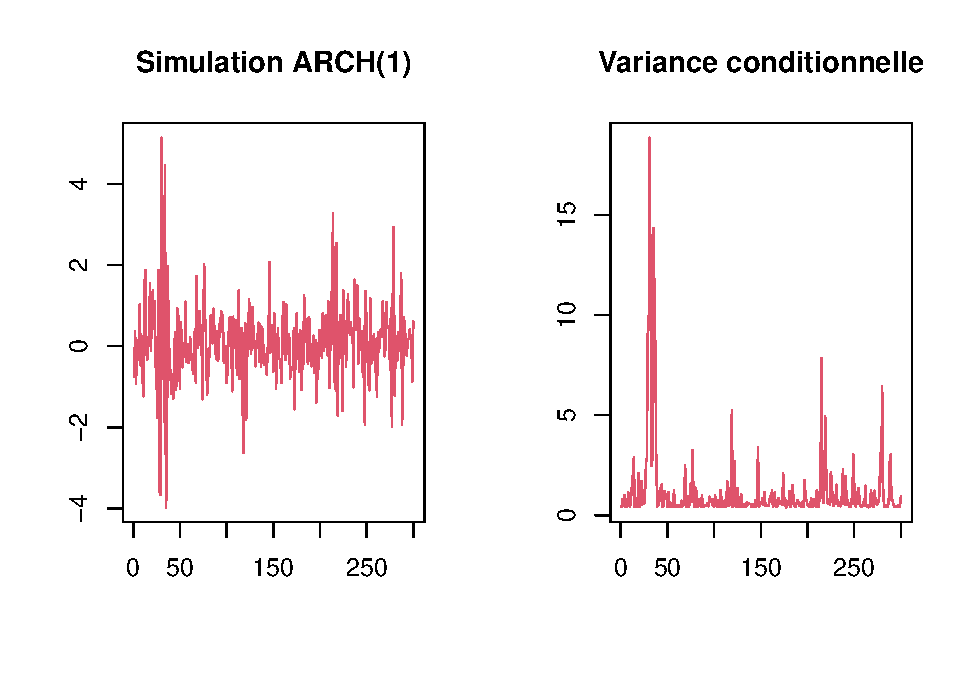
\includegraphics{chap2_files/figure-beamer/arch1Sim-1} \end{center}
\end{frame}
\begin{frame}{Propriétés statistiques}
\protect\hypertarget{propriuxe9tuxe9s-statistiques}{}
Soit \(X_t \sim ARCH(p)\). On a pour tout \(t\) et \(h \geq 1\),
\begin{itemize}[<+->]
\item
  \(\mathbb{E}\left(X_t|\mathcal{I}_{t-1} \right)=0\) et
  \(\mathbb{E}\left(X_t \right)=0\).
\item
  \(\mathbb{V}\left(X_t|\mathcal{I}_{t-1} \right)= \sigma^2_t, \; \forall t\)
  et
  \(\mathbb{V}\left(X_t \right)=\dfrac{a_0}{1-\displaystyle \sum_{i=1}^pa_i}\).
\item
  \(\mathbb{Cov}\left(X_t X_{t+h}|\mathcal{I}_{t-1} \right)=0\) pour
  \(h \geq 1\) et \(\mathbb{Cov}\left(X_t X_{t+h}\right)=0\).
\item
  \textbf{Rappel}
\item
  \(\mathbb{E}(X)=\mathbb{E}\big(\mathbb{E}(X|Y)\big)\).
\item
  Soit \(A_1 \subseteq A_2\),
  \(\mathbb{E}(X|A_1)=\mathbb{E}\big(\mathbb{E}(X|A_2)|A_1\big)\).
\end{itemize}
\end{frame}
\begin{frame}{La construction du modèle ARCH}
\protect\hypertarget{la-construction-du-moduxe8le-arch}{}
\begin{itemize}[<+->]
\item
  La construction du modèle ARCH passe par 4 étapes:
  \begin{enumerate}[<+->]
  \item
    Détermination de l'ordre \(p\).
  \item
    Estimation du modèle \(ARCH(p)\).
  \item
    Diagnostic du modèle estimé.
  \item
    Prévision.
  \end{enumerate}
\end{itemize}
\end{frame}
\begin{frame}
\textbf{Détermination de l'ordre} \(\mathbf{p}\)\textbf{:}
\begin{itemize}[<+->]
\item
  Similairement aux modèles ARMA, l'ordre \(p\) peut être déterminé en
  examinant la fonction d'auto-corrélation partielle de
  \(\varepsilon_t^2\).
\item
  On peut aussi faire recours aux critères de sélection: AIC, SIC et
  AICc.
\item
  \(AIC=-2logL+2k\), (Akaike information criteria) \(k=\) nombre de
  paramètres dans le modèle estimé.
\item
  \(BIC=-2logL+\log(T)k\). (Bayesian information criteria )
\item
  Pour un échantillon de petite taille, on utilise le critère \(AICc\)
  qui est défini par \[
  AICc=AIC+\dfrac{2k(k+1)}{T-k-1}
  \]
\end{itemize}
\end{frame}
\begin{frame}[fragile]
Reprenons notre exemple du chapitre précédent, les rendements du
bitcoin.
\begin{Shaded}
\begin{Highlighting}[]
\FunctionTok{library}\NormalTok{(quantmod); }\FunctionTok{library}\NormalTok{(zoo)}
\NormalTok{btc}\OtherTok{=}\FunctionTok{getSymbols}\NormalTok{(}\StringTok{"BTC{-}USD"}\NormalTok{, }\AttributeTok{src=}\StringTok{"yahoo"}\NormalTok{, }\AttributeTok{from=}\StringTok{"2014{-}09{-}17"}\NormalTok{,}\AttributeTok{to=}\StringTok{"2021{-}10{-}20"}\NormalTok{,}\AttributeTok{auto.assign =} \ConstantTok{FALSE}\NormalTok{)}
\NormalTok{closedAdj}\OtherTok{=}\FunctionTok{zoo}\NormalTok{(}\FunctionTok{na.omit}\NormalTok{(btc[,}\DecValTok{6}\NormalTok{])); rt}\OtherTok{=}\FunctionTok{diff}\NormalTok{(}\FunctionTok{log}\NormalTok{(closedAdj))}
\FunctionTok{pacf}\NormalTok{(rt}\SpecialCharTok{\^{}}\DecValTok{2}\NormalTok{,}\AttributeTok{na.action =}\NormalTok{ na.pass, }\AttributeTok{col=}\DecValTok{4}\NormalTok{, }\AttributeTok{xlab=}\StringTok{""}\NormalTok{)}
\end{Highlighting}
\end{Shaded}
\begin{center}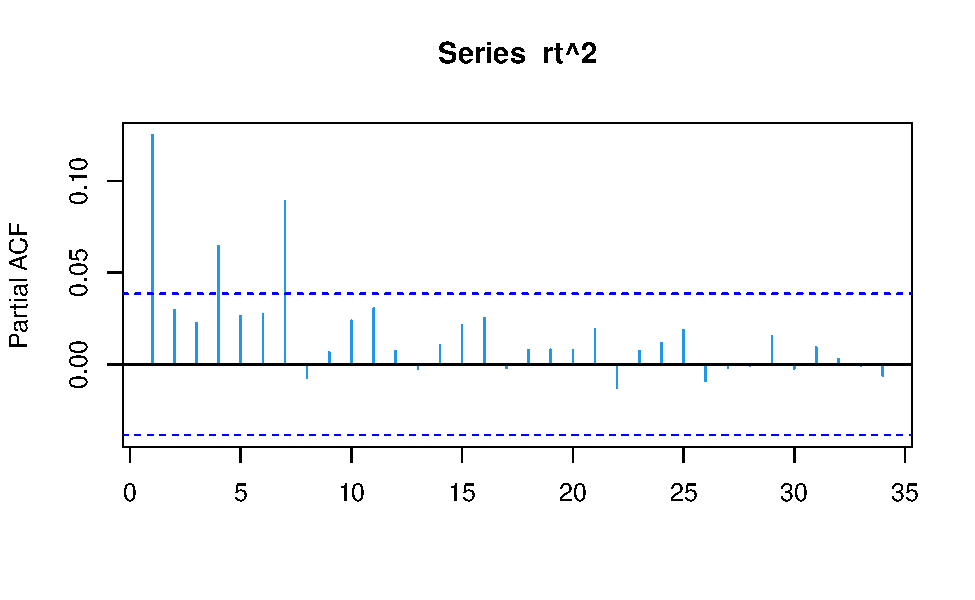
\includegraphics[width=0.8\linewidth]{chap2_files/figure-beamer/Rbtc-1} \end{center}
\end{frame}
\begin{frame}[fragile]
D'après le graphique de la fonction d'auto-corrélation partielle de
\(r_t^2\), on remarque bien que le modèle ARCH d'ordre 1 est approprié
aux rendements du BTC. On remarque aussi, que les pacf d'ordres 4 et 7
sont aussi significativement différents de zéro.
Déterminons les valeurs des critères d'information pour les modèles
ARCH(1) et ARCH(4).
Sous R, il existe plusieurs packages permettant l'estimation des modèles
GARCH tels que \texttt{tseries}, \texttt{fGarch}, \texttt{rugarch}.
Ici, nous décrivons l'utilisation des packages \texttt{fGarch} et
\texttt{rugarch}. Pour l'estimation du modèle ARCH, nous devons
spécifier le modèle à estimer en donnant les ordres des différents
modèles (mean and variance equations).
La fonction à utiliser est \texttt{ugarchspec} (\texttt{rugarch}) et
prend comme arguments principaux \texttt{variance.model},
\texttt{mean.model} et \texttt{distribution.model}. Les deux premiers
arguments sont des listes et le toisième est une chaîne de caractère qui
peut être \texttt{"norm"}, \texttt{"std"}, \texttt{"sstd} \texttt{"ged"}
ou \texttt{sged}.
\end{frame}
\begin{frame}[fragile]
\begin{Shaded}
\begin{Highlighting}[]
\FunctionTok{library}\NormalTok{(rugarch)   }\CommentTok{\# charger le package}
\NormalTok{spec1}\OtherTok{=}\FunctionTok{ugarchspec}\NormalTok{(}\AttributeTok{variance.model =} \FunctionTok{list}\NormalTok{(}\AttributeTok{garchOrder=}\FunctionTok{c}\NormalTok{(}\DecValTok{1}\NormalTok{,}\DecValTok{0}\NormalTok{)),}
                \AttributeTok{mean.model =} \FunctionTok{list}\NormalTok{(}\AttributeTok{armaOrder=}\FunctionTok{c}\NormalTok{(}\DecValTok{0}\NormalTok{,}\DecValTok{0}\NormalTok{)))}
\NormalTok{spec4}\OtherTok{=}\FunctionTok{ugarchspec}\NormalTok{(}\AttributeTok{variance.model =} \FunctionTok{list}\NormalTok{(}\AttributeTok{garchOrder=}\FunctionTok{c}\NormalTok{(}\DecValTok{4}\NormalTok{,}\DecValTok{0}\NormalTok{)),}
                \AttributeTok{mean.model =} \FunctionTok{list}\NormalTok{(}\AttributeTok{armaOrder=}\FunctionTok{c}\NormalTok{(}\DecValTok{0}\NormalTok{,}\DecValTok{0}\NormalTok{)))}
\NormalTok{fit1}\OtherTok{=}\FunctionTok{ugarchfit}\NormalTok{(spec1,rt)  }\CommentTok{\# Estimation}
\NormalTok{fit4}\OtherTok{=}\FunctionTok{ugarchfit}\NormalTok{(spec4,rt)}
\FunctionTok{t}\NormalTok{(}\FunctionTok{infocriteria}\NormalTok{(fit1))  }\CommentTok{\# critères d\textquotesingle{}information (normalisés)}
\end{Highlighting}
\end{Shaded}
\begin{verbatim}
    Akaike     Bayes   Shibata Hannan-Quinn
 0.5254326 0.5322282 0.5254299    0.5278955
\end{verbatim}
\begin{Shaded}
\begin{Highlighting}[]
\FunctionTok{t}\NormalTok{(}\FunctionTok{infocriteria}\NormalTok{(fit4))}
\end{Highlighting}
\end{Shaded}
\begin{verbatim}
   Akaike     Bayes   Shibata Hannan-Quinn
 -3.75665 -3.743059 -3.756661    -3.751724
\end{verbatim}
\end{frame}
\begin{frame}
\textbf{Estimation}
\begin{itemize}[<+->]
\item
  Sous l'hypothèse de normalité des erreurs, la fonction de
  vraisemblance d'un modèle \(ARCH(p)\) est: \[
  L(\varepsilon_1, \varepsilon_2,\ldots,\varepsilon_T|\mathbf{a})=\prod_{i=p+1}^T\dfrac{1}{\sqrt{2\pi\sigma^2_t}}\exp{\left(-\dfrac{\varepsilon_t^2}{2\sigma^2_t} \right)}\times f(\varepsilon_1, \varepsilon_2,\ldots,\varepsilon_T|\mathbf{a})
  \] où \(\mathbf{a}=(a_0,a_1,\ldots,a_p)\) et
  \(f(\varepsilon_1, \varepsilon_2,\ldots,\varepsilon_T|\mathbf{a})\) la
  densité conjointe conditionnelle des erreurs.
\item
  Maximiser la fonction de vraisemblance conditionnelle est équivalent à
  maximiser son logarithme. Le logarithme de la vraisemblance
  conditionnelle est: \[
  \ell(\varepsilon_{\color{red}{p+1}}, \varepsilon_\color{red}{{p+2}},\ldots,\varepsilon_\color{red}{T}|\mathbf{a}, a_\color{red}{1},a_\color{red}{2},\ldots,a_\color{red}{p})=\sum_{i=p+1}^T\left[-\frac{1}{2}\log(2\pi)-\frac{1}{2}\log(\sigma^2_t)-\frac{1}{2}\frac{\varepsilon_t^2}{\sigma^2_t} \right]
  \] où
  \(\sigma^2_t=a_0+a_1\varepsilon^2_{t-1}+a_2\varepsilon^2_{t-2}+\ldots+a_p\varepsilon^2_{t-p}\)
  qui peut être calculé récursivement.
\item
  \textbf{Remarque:} On peut aussi utiliser d'autres distributions autre
  que la loi normale telles que la loi de student ou la loi GED
  (Generalized Error Distribution).
\end{itemize}
\end{frame}
\begin{frame}
\textbf{Exemple:} Soit \(X_t \sim ARCH(1)\). Donner les estimateurs de
\(\mu\), \(a_0\), et \(a_1\) par la méthode de MV.
\begin{itemize}[<+->]
\tightlist
\item
  Le logarithme de la vraisemblance conditionnelle est donnée par: \[
  \ell(\varepsilon_{2}, \varepsilon_{3},\ldots,\varepsilon_T|\mathbf{a}, a_1,a_2)=\sum_{i=2}^T\left[-\frac{1}{2}\log(2\pi)-\frac{1}{2}\log(a_0+a_1X^2_{t-1})-\frac{1}{2}\frac{(X_t-\mu)^2}{a_0+a_1X^2_{t-1}} \right]
  \] Les paramètres \(\mu\), \(a_0\) et \(a_1\) se déduisent en
  résolvant le système suivant \[
  \begin{cases}
  \frac{\partial \ell}{\partial \mu}=0 \\
  \frac{\partial \ell}{\partial a_0}=0 \\
  \frac{\partial \ell}{\partial a_1}=0 
  \end{cases}
  \]
\end{itemize}
\end{frame}
\begin{frame}[fragile]
\begin{Shaded}
\begin{Highlighting}[]
\NormalTok{fit1}\SpecialCharTok{@}\NormalTok{fit}\SpecialCharTok{$}\NormalTok{matcoef}
\end{Highlighting}
\end{Shaded}
\begin{verbatim}
           Estimate   Std. Error     t value    Pr(>|t|)
mu     1.774978e-01 5.624388e-05 3155.859739 0.000000000
omega  1.470274e-06 4.864592e-07    3.022399 0.002507798
alpha1 5.665866e-01 1.517078e-04 3734.722111 0.000000000
\end{verbatim}
\begin{Shaded}
\begin{Highlighting}[]
\FunctionTok{show}\NormalTok{(fit1)}
\end{Highlighting}
\end{Shaded}
\begin{verbatim}
*---------------------------------*
*          GARCH Model Fit        *
*---------------------------------*
Conditional Variance Dynamics   
-----------------------------------
GARCH Model : sGARCH(1,0)
Mean Model  : ARFIMA(0,0,0)
Distribution    : norm 
Optimal Parameters
------------------------------------
        Estimate  Std. Error   t value Pr(>|t|)
mu      0.177498    0.000056 3155.8597 0.000000
omega   0.000001    0.000000    3.0224 0.002508
alpha1  0.566587    0.000152 3734.7221 0.000000
Robust Standard Errors:
        Estimate  Std. Error  t value Pr(>|t|)
mu      0.177498    22.55445 0.007870  0.99372
omega   0.000001     0.11523 0.000013  0.99999
alpha1  0.566587    63.19311 0.008966  0.99285
LogLikelihood : -676.3843 
Information Criteria
------------------------------------
                    
Akaike       0.52543
Bayes        0.53223
Shibata      0.52543
Hannan-Quinn 0.52790
Weighted Ljung-Box Test on Standardized Residuals
------------------------------------
                        statistic   p-value
Lag[1]                      52.71 3.874e-13
Lag[2*(p+q)+(p+q)-1][2]     52.71 1.221e-14
Lag[4*(p+q)+(p+q)-1][5]     53.72 5.440e-15
d.o.f=0
H0 : No serial correlation
Weighted Ljung-Box Test on Standardized Squared Residuals
------------------------------------
                        statistic p-value
Lag[1]                    0.00174  0.9667
Lag[2*(p+q)+(p+q)-1][2]   0.00462  0.9948
Lag[4*(p+q)+(p+q)-1][5]   0.01041  1.0000
d.o.f=1
Weighted ARCH LM Tests
------------------------------------
            Statistic Shape Scale P-Value
ARCH Lag[2]   0.00575 0.500 2.000  0.9396
ARCH Lag[4]   0.01068 1.397 1.611  0.9993
ARCH Lag[6]   0.02494 2.222 1.500  1.0000
Nyblom stability test
------------------------------------
Joint Statistic:  1.2607
Individual Statistics:              
mu     0.09819
omega  0.07014
alpha1 0.09821
Asymptotic Critical Values (10% 5% 1%)
Joint Statistic:         0.846 1.01 1.35
Individual Statistic:    0.35 0.47 0.75
Sign Bias Test
------------------------------------
                   t-value      prob sig
Sign Bias            5.257 1.584e-07 ***
Negative Sign Bias   8.921 8.550e-19 ***
Positive Sign Bias   3.554 3.863e-04 ***
Joint Effect       124.060 1.030e-26 ***
Adjusted Pearson Goodness-of-Fit Test:
------------------------------------
  group statistic p-value(g-1)
1    20     11426            0
2    30     11779            0
3    40     11946            0
4    50     12052            0
Elapsed time : 0.2354479 
\end{verbatim}
\end{frame}
\begin{frame}
\begin{itemize}[<+->]
\tightlist
\item
  Le modèle estimé est alors:
\end{itemize}
\[
\begin{cases}
X_t=0.1775+\sigma_t \varepsilon_t\\
\sigma^2_t=1.4702 \times 10^{-6}+0.56658\; X^2_{t-1}
\end{cases}
\]
\end{frame}
\begin{frame}[fragile]
\begin{itemize}[<+->]
\item
  Estimation avec des erreurs de loi de student:
\item
  Tout d'abord, examinons la distribution des erreurs et la comparons
  par la densité normale.
\end{itemize}
\begin{Shaded}
\begin{Highlighting}[]
\FunctionTok{hist}\NormalTok{(rt,}\AttributeTok{col=}\DecValTok{4}\NormalTok{, }\AttributeTok{prob=}\NormalTok{T, }\AttributeTok{breaks =} \DecValTok{50}\NormalTok{) }\CommentTok{\# histogramme or rt}
\FunctionTok{lines}\NormalTok{(}\FunctionTok{density}\NormalTok{(rt), }\AttributeTok{col=}\DecValTok{2}\NormalTok{,}\AttributeTok{lwd=}\DecValTok{3}\NormalTok{) }\CommentTok{\# density estimation (kernel)}
\FunctionTok{curve}\NormalTok{(}\FunctionTok{dnorm}\NormalTok{(x, }\FunctionTok{mean}\NormalTok{(rt),}\FunctionTok{sd}\NormalTok{(rt)), }\AttributeTok{lwd=}\DecValTok{3}\NormalTok{, }\AttributeTok{col=}\StringTok{"darkorchid3"}\NormalTok{, }\AttributeTok{add=}\NormalTok{T) }\CommentTok{\# normal density}
\FunctionTok{legend}\NormalTok{(}\StringTok{"topleft"}\NormalTok{,}\AttributeTok{bty=}\StringTok{"n"}\NormalTok{,}\AttributeTok{lwd=}\DecValTok{3}\NormalTok{, }\AttributeTok{col=}\FunctionTok{c}\NormalTok{(}\DecValTok{2}\NormalTok{,}\StringTok{"darkorchid3"}\NormalTok{),}
       \AttributeTok{legend=}\FunctionTok{c}\NormalTok{(}\StringTok{"Kernel"}\NormalTok{,}\StringTok{"Normal"}\NormalTok{))}
\end{Highlighting}
\end{Shaded}
\end{frame}
\begin{frame}
\begin{center}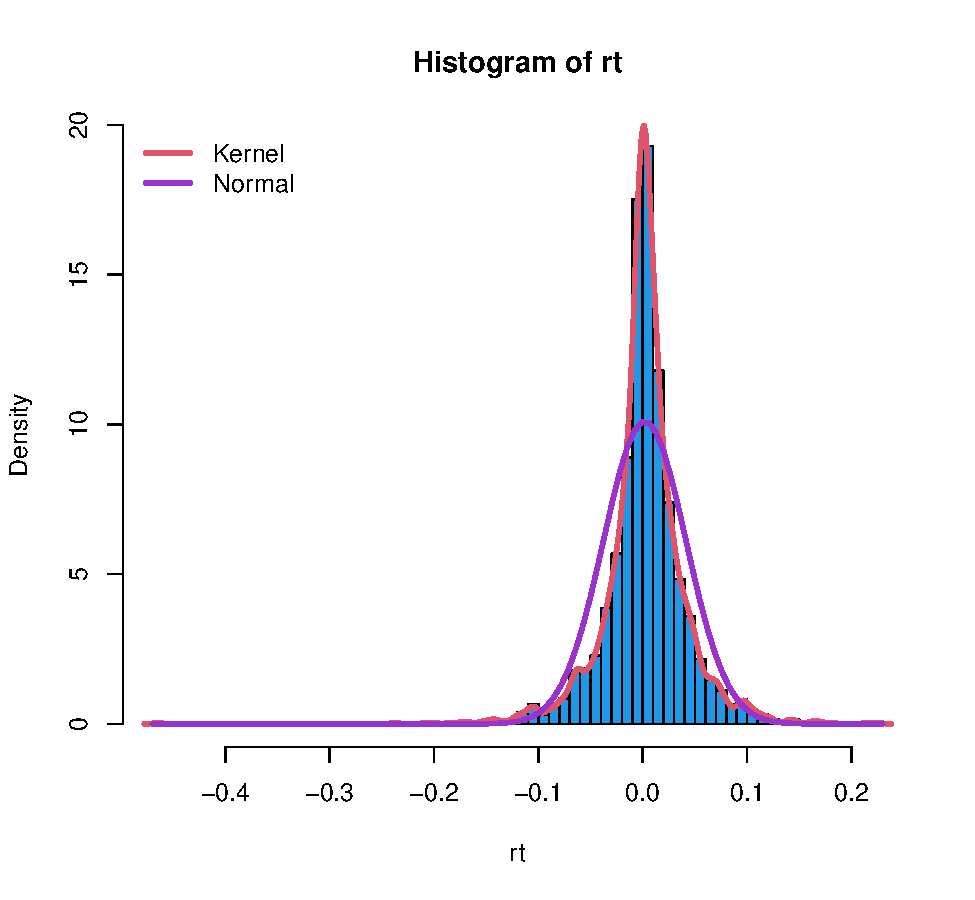
\includegraphics[width=0.8\linewidth]{chap2_files/figure-beamer/hist_rt2-1} \end{center}
\end{frame}
\begin{frame}[fragile]
\begin{Shaded}
\begin{Highlighting}[]
\NormalTok{specSt}\OtherTok{=}\FunctionTok{ugarchspec}\NormalTok{(}\FunctionTok{list}\NormalTok{(}\AttributeTok{garchOrder=}\FunctionTok{c}\NormalTok{(}\DecValTok{1}\NormalTok{,}\DecValTok{0}\NormalTok{)), }\FunctionTok{list}\NormalTok{(}\AttributeTok{armaOrder=}\FunctionTok{c}\NormalTok{(}\DecValTok{0}\NormalTok{,}\DecValTok{0}\NormalTok{)),}\AttributeTok{distribution.model =} \StringTok{"std"}\NormalTok{)}
\NormalTok{fitst}\OtherTok{=}\FunctionTok{ugarchfit}\NormalTok{(specSt,rt)}
\FunctionTok{show}\NormalTok{(fitst)}
\end{Highlighting}
\end{Shaded}
\begin{verbatim}
*---------------------------------*
*          GARCH Model Fit        *
*---------------------------------*
Conditional Variance Dynamics   
-----------------------------------
GARCH Model : sGARCH(1,0)
Mean Model  : ARFIMA(0,0,0)
Distribution    : std 
Optimal Parameters
------------------------------------
        Estimate  Std. Error  t value Pr(>|t|)
mu      0.002287    0.000474   4.8272 0.000001
omega   0.002465    0.000820   3.0058 0.002649
alpha1  0.999000    0.380806   2.6234 0.008706
shape   2.291507    0.123369  18.5745 0.000000
Robust Standard Errors:
        Estimate  Std. Error  t value Pr(>|t|)
mu      0.002287    0.000486   4.7104 0.000002
omega   0.002465    0.000794   3.1057 0.001898
alpha1  0.999000    0.459204   2.1755 0.029592
shape   2.291507    0.138161  16.5858 0.000000
LogLikelihood : 5134.626 
Information Criteria
------------------------------------
                    
Akaike       -3.9680
Bayes        -3.9589
Shibata      -3.9680
Hannan-Quinn -3.9647
Weighted Ljung-Box Test on Standardized Residuals
------------------------------------
                        statistic p-value
Lag[1]                      1.139  0.2858
Lag[2*(p+q)+(p+q)-1][2]     1.412  0.3819
Lag[4*(p+q)+(p+q)-1][5]     2.774  0.4500
d.o.f=0
H0 : No serial correlation
Weighted Ljung-Box Test on Standardized Squared Residuals
------------------------------------
                        statistic p-value
Lag[1]                      1.113  0.2914
Lag[2*(p+q)+(p+q)-1][2]     1.141  0.4548
Lag[4*(p+q)+(p+q)-1][5]     4.098  0.2421
d.o.f=1
Weighted ARCH LM Tests
------------------------------------
            Statistic Shape Scale P-Value
ARCH Lag[2]   0.05445 0.500 2.000  0.8155
ARCH Lag[4]   3.38062 1.397 1.611  0.2142
ARCH Lag[6]   5.23590 2.222 1.500  0.1724
Nyblom stability test
------------------------------------
Joint Statistic:  5.1393
Individual Statistics:             
mu     0.2772
omega  3.5836
alpha1 0.2891
shape  2.6941
Asymptotic Critical Values (10% 5% 1%)
Joint Statistic:         1.07 1.24 1.6
Individual Statistic:    0.35 0.47 0.75
Sign Bias Test
------------------------------------
                   t-value   prob sig
Sign Bias           0.3356 0.7372    
Negative Sign Bias  1.5122 0.1306    
Positive Sign Bias  1.6918 0.0908   *
Joint Effect        5.6371 0.1307    
Adjusted Pearson Goodness-of-Fit Test:
------------------------------------
  group statistic p-value(g-1)
1    20     65.91    4.340e-07
2    30     82.56    4.856e-07
3    40     95.67    1.153e-06
4    50    103.17    9.845e-06
Elapsed time : 0.628963 
\end{verbatim}
\end{frame}
\begin{frame}[fragile]
\textbf{Diagnostique du modèle estimé}
\begin{itemize}[<+->]
\item
  Pour un modèle ARCH bien approprié, les erreurs standards
  \(\widetilde{\varepsilon}_t=\frac{\varepsilon_t}{\sigma_t}\) doivent
  être \(iid\). La statistique de Ljung-Box peut être appliqué sur les
  erreurs standards (\(\widetilde{\varepsilon}_t\)) pour examiner
  l'équation de la moyenne conditionnelle et sur leurs carrés
  (\(\widetilde{\varepsilon}_t^2\)) pour examiner l'équation de la
  variance conditionnelle.
\item
  Lest tests de stochasticité (randomness tests) peuvent être aussi
  appliqué tels que le test BDS, run test, etc\ldots{}
\item
  Le package \texttt{rugarch} utilise plutôt les statistiques de
  Ljung-Box pondérée et LM-ARCH pondérée proposé par (Fisher and
  Gallagher 2012)
\item
  Le package \texttt{fGarch} utilise les statistiques de Ljung-Box et
  LM-ARCH standards sur les erreurs standards et leurs carrés.
\end{itemize}
\end{frame}
\begin{frame}[fragile]
\begin{Shaded}
\begin{Highlighting}[]
\FunctionTok{library}\NormalTok{(fGarch)}
\NormalTok{fitst2}\OtherTok{=}\FunctionTok{garchFit}\NormalTok{(}\SpecialCharTok{\textasciitilde{}}\FunctionTok{garch}\NormalTok{(}\DecValTok{1}\NormalTok{,}\DecValTok{0}\NormalTok{),rt, }\AttributeTok{cond.dist =} \StringTok{"std"}\NormalTok{, }\AttributeTok{trace =}\NormalTok{ F )}
\end{Highlighting}
\end{Shaded}
\begin{verbatim}
Warning: Using formula(x) is deprecated when x is a character vector of length > 1.
  Consider formula(paste(x, collapse = " ")) instead.
\end{verbatim}
\begin{Shaded}
\begin{Highlighting}[]
\NormalTok{fitst2}\SpecialCharTok{@}\NormalTok{fit}\SpecialCharTok{$}\NormalTok{matcoef   }\CommentTok{\# fGarch}
\end{Highlighting}
\end{Shaded}
\begin{verbatim}
          Estimate   Std. Error   t value     Pr(>|t|)
mu     0.002290206 0.0004739852  4.831808 1.352984e-06
omega  0.002509288 0.0008199825  3.060172 2.212096e-03
alpha1 0.999999990 0.3677348660  2.719350 6.541026e-03
shape  2.286381480 0.1179821323 19.379049 0.000000e+00
\end{verbatim}
\begin{Shaded}
\begin{Highlighting}[]
\NormalTok{fitst}\SpecialCharTok{@}\NormalTok{fit}\SpecialCharTok{$}\NormalTok{matcoef    }\CommentTok{\# rugarch}
\end{Highlighting}
\end{Shaded}
\begin{verbatim}
          Estimate   Std. Error   t value     Pr(>|t|)
mu     0.002287490 0.0004738717  4.827234 1.384422e-06
omega  0.002465219 0.0008201576  3.005787 2.648943e-03
alpha1 0.998999883 0.3808058193  2.623384 8.706109e-03
shape  2.291507174 0.1233687554 18.574453 0.000000e+00
\end{verbatim}
\end{frame}
\begin{frame}[fragile]
\begin{Shaded}
\begin{Highlighting}[]
\FunctionTok{summary}\NormalTok{(fitst2)}
\end{Highlighting}
\end{Shaded}
\begin{verbatim}
Title:
 GARCH Modelling 
Call:
 garchFit(formula = ~garch(1, 0), data = rt, cond.dist = "std", 
    trace = F) 
Mean and Variance Equation:
 data ~ garch(1, 0)
<environment: 0x0000000034aef4d8>
 [data = rt]
Conditional Distribution:
 std 
Coefficient(s):
       mu      omega     alpha1      shape  
0.0022902  0.0025093  1.0000000  2.2863815  
Std. Errors:
 based on Hessian 
Error Analysis:
        Estimate  Std. Error  t value Pr(>|t|)    
mu      0.002290    0.000474    4.832 1.35e-06 ***
omega   0.002509    0.000820    3.060  0.00221 ** 
alpha1  1.000000    0.367735    2.719  0.00654 ** 
shape   2.286382    0.117982   19.379  < 2e-16 ***
---
Signif. codes:  0 '***' 0.001 '**' 0.01 '*' 0.05 '.' 0.1 ' ' 1
Log Likelihood:
 5135.542    normalized:  1.985902 
Description:
 Mon Nov 01 23:16:58 2021 by user: User 
Standardised Residuals Tests:
                                Statistic p-Value     
 Jarque-Bera Test   R    Chi^2  36280.16  0           
 Shapiro-Wilk Test  R    W      0.8861145 0           
 Ljung-Box Test     R    Q(10)  21.09798  0.02042062  
 Ljung-Box Test     R    Q(15)  22.20446  0.1025538   
 Ljung-Box Test     R    Q(20)  29.7996   0.07316659  
 Ljung-Box Test     R^2  Q(10)  36.2839   7.522355e-05
 Ljung-Box Test     R^2  Q(15)  38.19344  0.0008447584
 Ljung-Box Test     R^2  Q(20)  39.7931   0.005304967 
 LM Arch Test       R    TR^2   36.09029  0.0003133419
Information Criterion Statistics:
      AIC       BIC       SIC      HQIC 
-3.968710 -3.959649 -3.968715 -3.965426 
\end{verbatim}
\end{frame}
\begin{frame}
\textbf{Prévision}
\begin{itemize}[<+->]
\item
  Les prévisions du model ARCH est obtenues récursivement comme celles
  du modèle AR.
\item
  La prévision à une étape est
  \(\sigma^2_h(1)=a_0+a_1 \varepsilon^2_h+\ldots+a_p \varepsilon^2_{h+1-p}\).
\item
  La prévision à deux étapes est
  \(\sigma^2_h(2)=a_0+a_1 \sigma^2_h(1)+a_2\varepsilon^2_h+\ldots+a_p \varepsilon^2_{h+2-p}\).
\item
  La prévision à \(k\) étapes est
  \(\sigma^2_h(k)=a_0+\displaystyle \sum_{j=1}^pa_j\sigma^2_h(k-j)\) où
  \(\sigma^2_h(k-j)=\varepsilon^2_{h+k-1}\) si \(k-j \leq 0\).
\end{itemize}
\end{frame}
\begin{frame}[fragile]
\begin{Shaded}
\begin{Highlighting}[]
\FunctionTok{predict}\NormalTok{(fitst2,}\DecValTok{3}\NormalTok{)           }\CommentTok{\# fGarch}
\end{Highlighting}
\end{Shaded}
\begin{verbatim}
  meanForecast  meanError standardDeviation
1  0.002290206 0.05567025        0.05567025
2  0.002290206 0.07488968        0.07488968
3  0.002290206 0.09009857        0.09009857
\end{verbatim}
\begin{Shaded}
\begin{Highlighting}[]
\FunctionTok{ugarchforecast}\NormalTok{(fitst, }\AttributeTok{n.ahead=}\DecValTok{3}\NormalTok{)    }\CommentTok{\# rugarch}
\end{Highlighting}
\end{Shaded}
\begin{verbatim}
*------------------------------------*
*       GARCH Model Forecast         *
*------------------------------------*
Model: sGARCH
Horizon: 3
Roll Steps: 0
Out of Sample: 0
0-roll forecast [T0=2021-10-20]:
      Series   Sigma
T+1 0.002287 0.05527
T+2 0.002287 0.07428
T+3 0.002287 0.08931
\end{verbatim}
\end{frame}
\begin{frame}
\begin{itemize}[<+->]
\item
  Calcul des prévisions à la main:
\item
  On a \(\widehat{\varepsilon}_T=5.9002 \times 10^{-4}\), déterminons
  \(\widehat{\sigma}^2_T(k)\), \(k=1,2,3\).
\item
  \(\widehat{\sigma}^2_T(1)=a_0+a_1 \varepsilon^2_h=2.467 \times 10^{-3}+1\times 5.9002 \times 10^{-4}=0.00305702\).
\item
  \(\widehat{\sigma}^2_T(2)=a_0+a_1 \widehat{\sigma}^2_T(1)=2.467 \times 10^{-3}+1\times 3.057 \times 10^{-3}=0.005524\).
\item
  \(\widehat{\sigma}^2_T(3)=a_0+a_1 \widehat{\sigma}^2_T(2)=2.467 \times 10^{-3}+1\times 5.524 \times 10^{-3}=0.007991\).
\end{itemize}
\end{frame}
\begin{frame}{Le modèle GARCH}
\protect\hypertarget{le-moduxe8le-garch}{}
\begin{itemize}[<+->]
\item
  Le modèle GARCH (\emph{Generalized ARCH}) est proposé par (Bollerslev
  1986).
\item
  \(X_t\sim GARCH(p,q)\) si \(X_t=\varepsilon_t=\sigma_tZ_t\) et
  \(\sigma^2_t=a_0+\displaystyle \sum_{i=1}^pa_i\varepsilon^2_{t-i}+\displaystyle \sum_{j=1}^q\beta_j\sigma^2_{t-j}\)
  où \(Z_t \stackrel{iid}{\sim}N(0,1)\), \(a0 >0\), \(a_i \geq 0\),
  \(\beta_j \geq 0\) et
  \(\displaystyle \sum_{i=1}^{\max(p,q)}(a_i+\beta_j) < 1\).
\item
  La dernière contrainte implique que la variance inconditionnelle de
  \(X_t\) est finie et que sa variance conditionnelle varie en fonction
  du temps.
\item
  La prévision du modèle GARCH se fait similairement à un modèle ARMA.
  Soit \(X_t=\sigma_t Z_t\) et
  \(\sigma^2_t=a_0+a_1 \varepsilon^2_{t-1}+\beta_1\sigma^2_{t-1}\). On a
  alors:
\item
  \(\sigma_h(1)=a_0+a_1\varepsilon^2_h+\beta_1\sigma^2_h\),
\item
  \(\sigma_h(2)=a_0+(a_1+\beta_1)\sigma^2_h(1)+a_1\sigma^2_h(1)(Z^2_{h+1}-1)\)
  et puisque \(\mathbb{E}(Z^2_{h+1}-1|\mathcal{I}_h)=0\), alors
  \(\sigma_h(2)=a_0+(a_1+\beta_1)\sigma^2_h(1)\)
\item
  Et de manière générale, \(\sigma_h(k)=a_0+(a_1+\beta_1)\sigma^2_h(k)\)
\end{itemize}
\end{frame}
\begin{frame}
\textbf{Remarques:}
\begin{itemize}[<+->]
\item
  En générale, les modèles GARCH s'appliquent aux erreurs suite à un
  modèle linéaire (régression linéaire, ARMA).
\item
  Comme dans le modèle ARCH, les erreurs \(Z_t\) dans le modèle GARCH
  peuvent être de loi Student ou GED.
\item
  La détermination de l'ordre \(q\) du modèle GARCH se base sur la
  fonction d'auto-corrélation de \(X_t^2\).
\item
  Estimons les rendements du BTC à l'aide d'un modèle GARCH(1,1).
\end{itemize}
\end{frame}
\begin{frame}[fragile]
\begin{Shaded}
\begin{Highlighting}[]
\NormalTok{garch11}\OtherTok{=}\FunctionTok{garchFit}\NormalTok{(}\SpecialCharTok{\textasciitilde{}}\FunctionTok{garch}\NormalTok{(}\DecValTok{1}\NormalTok{,}\DecValTok{1}\NormalTok{),rt, }\AttributeTok{trace =}\NormalTok{ F)   }\CommentTok{\#fGarch}
\NormalTok{garch11}\SpecialCharTok{@}\NormalTok{fit}\SpecialCharTok{$}\NormalTok{matcoef}
\end{Highlighting}
\end{Shaded}
\begin{verbatim}
           Estimate   Std. Error   t value     Pr(>|t|)
mu     2.182371e-03 6.334182e-04  3.445387 5.702419e-04
omega  6.937465e-05 1.063513e-05  6.523160 6.884138e-11
alpha1 1.339155e-01 1.523577e-02  8.789549 0.000000e+00
beta1  8.365670e-01 1.548134e-02 54.037112 0.000000e+00
\end{verbatim}
\begin{Shaded}
\begin{Highlighting}[]
\NormalTok{spec11}\OtherTok{=}\FunctionTok{ugarchspec}\NormalTok{(}\AttributeTok{variance.model =} \FunctionTok{list}\NormalTok{(}\AttributeTok{garchOrder=}\FunctionTok{c}\NormalTok{(}\DecValTok{1}\NormalTok{,}\DecValTok{1}\NormalTok{)),}
                  \AttributeTok{mean.model =} \FunctionTok{list}\NormalTok{(}\AttributeTok{armaOrder=}\FunctionTok{c}\NormalTok{(}\DecValTok{0}\NormalTok{,}\DecValTok{0}\NormalTok{)))}
\NormalTok{Garch11}\OtherTok{=}\FunctionTok{ugarchfit}\NormalTok{(spec11,rt)}
\NormalTok{Garch11}\SpecialCharTok{@}\NormalTok{fit}\SpecialCharTok{$}\NormalTok{matcoef}
\end{Highlighting}
\end{Shaded}
\begin{verbatim}
           Estimate   Std. Error   t value     Pr(>|t|)
mu     2.182108e-03 6.334382e-04  3.444864 5.713467e-04
omega  6.933686e-05 1.066024e-05  6.504249 7.808243e-11
alpha1 1.337894e-01 1.523686e-02  8.780639 0.000000e+00
beta1  8.366535e-01 1.551168e-02 53.937005 0.000000e+00
\end{verbatim}
\end{frame}
\begin{frame}[fragile]
\begin{verbatim}
Title:
 GARCH Modelling 
Call:
 garchFit(formula = ~garch(1, 1), data = rt, trace = F) 
Mean and Variance Equation:
 data ~ garch(1, 1)
<environment: 0x0000000034cf1f20>
 [data = rt]
Conditional Distribution:
 norm 
Coefficient(s):
        mu       omega      alpha1       beta1  
2.1824e-03  6.9375e-05  1.3392e-01  8.3657e-01  
Std. Errors:
 based on Hessian 
Error Analysis:
        Estimate  Std. Error  t value Pr(>|t|)    
mu     2.182e-03   6.334e-04    3.445  0.00057 ***
omega  6.937e-05   1.064e-05    6.523 6.88e-11 ***
alpha1 1.339e-01   1.524e-02    8.790  < 2e-16 ***
beta1  8.366e-01   1.548e-02   54.037  < 2e-16 ***
---
Signif. codes:  0 '***' 0.001 '**' 0.01 '*' 0.05 '.' 0.1 ' ' 1
Log Likelihood:
 4910.658    normalized:  1.89894 
Description:
 Mon Nov 01 23:16:59 2021 by user: User 
Standardised Residuals Tests:
                                Statistic p-Value    
 Jarque-Bera Test   R    Chi^2  21488.29  0          
 Shapiro-Wilk Test  R    W      0.8992033 0          
 Ljung-Box Test     R    Q(10)  29.43062  0.001060873
 Ljung-Box Test     R    Q(15)  31.22058  0.008206586
 Ljung-Box Test     R    Q(20)  37.26145  0.01088514 
 Ljung-Box Test     R^2  Q(10)  3.238863  0.9752308  
 Ljung-Box Test     R^2  Q(15)  4.254493  0.9967773  
 Ljung-Box Test     R^2  Q(20)  5.188875  0.9996305  
 LM Arch Test       R    TR^2   3.432893  0.9916394  
Information Criterion Statistics:
      AIC       BIC       SIC      HQIC 
-3.794786 -3.785725 -3.794791 -3.791502 
\end{verbatim}
\end{frame}
\begin{frame}[fragile]
\begin{Shaded}
\begin{Highlighting}[]
\FunctionTok{show}\NormalTok{(Garch11)}
\end{Highlighting}
\end{Shaded}
\begin{verbatim}
*---------------------------------*
*          GARCH Model Fit        *
*---------------------------------*
Conditional Variance Dynamics   
-----------------------------------
GARCH Model : sGARCH(1,1)
Mean Model  : ARFIMA(0,0,0)
Distribution    : norm 
Optimal Parameters
------------------------------------
        Estimate  Std. Error  t value Pr(>|t|)
mu      0.002182    0.000633   3.4449 0.000571
omega   0.000069    0.000011   6.5042 0.000000
alpha1  0.133789    0.015237   8.7806 0.000000
beta1   0.836654    0.015512  53.9370 0.000000
Robust Standard Errors:
        Estimate  Std. Error  t value Pr(>|t|)
mu      0.002182    0.000729   2.9930 0.002762
omega   0.000069    0.000026   2.6688 0.007612
alpha1  0.133789    0.036614   3.6540 0.000258
beta1   0.836654    0.027806  30.0894 0.000000
LogLikelihood : 4910.635 
Information Criteria
------------------------------------
                    
Akaike       -3.7948
Bayes        -3.7857
Shibata      -3.7948
Hannan-Quinn -3.7915
Weighted Ljung-Box Test on Standardized Residuals
------------------------------------
                        statistic p-value
Lag[1]                      4.384 0.03628
Lag[2*(p+q)+(p+q)-1][2]     4.936 0.04230
Lag[4*(p+q)+(p+q)-1][5]     7.615 0.03669
d.o.f=0
H0 : No serial correlation
Weighted Ljung-Box Test on Standardized Squared Residuals
------------------------------------
                        statistic p-value
Lag[1]                  9.538e-07  0.9992
Lag[2*(p+q)+(p+q)-1][5] 1.372e+00  0.7714
Lag[4*(p+q)+(p+q)-1][9] 1.936e+00  0.9125
d.o.f=2
Weighted ARCH LM Tests
------------------------------------
            Statistic Shape Scale P-Value
ARCH Lag[3]    0.8783 0.500 2.000  0.3487
ARCH Lag[5]    1.7162 1.440 1.667  0.5374
ARCH Lag[7]    1.7975 2.315 1.543  0.7601
Nyblom stability test
------------------------------------
Joint Statistic:  0.9753
Individual Statistics:              
mu     0.27019
omega  0.36813
alpha1 0.08751
beta1  0.25175
Asymptotic Critical Values (10% 5% 1%)
Joint Statistic:         1.07 1.24 1.6
Individual Statistic:    0.35 0.47 0.75
Sign Bias Test
------------------------------------
                   t-value   prob sig
Sign Bias           0.8603 0.3897    
Negative Sign Bias  0.5948 0.5520    
Positive Sign Bias  0.4544 0.6496    
Joint Effect        1.7634 0.6229    
Adjusted Pearson Goodness-of-Fit Test:
------------------------------------
  group statistic p-value(g-1)
1    20     392.4    1.649e-71
2    30     429.5    7.774e-73
3    40     431.9    9.983e-68
4    50     462.6    1.103e-68
Elapsed time : 0.153199 
\end{verbatim}
\end{frame}
\begin{frame}[fragile]
\begin{Shaded}
\begin{Highlighting}[]
\FunctionTok{ugarchforecast}\NormalTok{(Garch11,}\AttributeTok{n.ahead =} \DecValTok{5}\NormalTok{)}
\end{Highlighting}
\end{Shaded}
\begin{verbatim}
*------------------------------------*
*       GARCH Model Forecast         *
*------------------------------------*
Model: sGARCH
Horizon: 5
Roll Steps: 0
Out of Sample: 0
0-roll forecast [T0=2021-10-20]:
      Series   Sigma
T+1 0.002182 0.03436
T+2 0.002182 0.03486
T+3 0.002182 0.03534
T+4 0.002182 0.03579
T+5 0.002182 0.03623
\end{verbatim}
\end{frame}
\begin{frame}
\textbf{Références}
\hypertarget{refs}{}
\begin{CSLReferences}{1}{0}
\leavevmode\vadjust pre{\hypertarget{ref-boll86}{}}%
Bollerslev, Tim. 1986. {``Generalized Autoregressive Conditional
Heteroskedasticity.''} \emph{Journal of Econometrics} 31 (3): 307--27.
https://doi.org/\url{https://doi.org/10.1016/0304-4076(86)90063-1}.
\leavevmode\vadjust pre{\hypertarget{ref-engle82}{}}%
Engle, Robert F. 1982. {``Autoregressive Conditional Heteroscedasticity
with Estimates of the Variance of United Kingdom Inflation.''}
\emph{Econometrica} 50 (4): 987--1007.
\leavevmode\vadjust pre{\hypertarget{ref-Fisher12}{}}%
Fisher, Thomas J., and Colin M. Gallagher. 2012. {``New Weighted
Portmanteau Statistics for Time Series Goodness of Fit Testing.''}
\emph{Journal of the American Statistical Association} 107 (498):
777--87. \url{https://doi.org/10.1080/01621459.2012.688465}.
\end{CSLReferences}
\end{frame}
\end{document}
